\documentclass[12pt]{article}

\pagestyle{empty}
\setlength{\topmargin}{0in}
\setlength{\headheight}{0in}
\setlength{\topsep}{0in}
\setlength{\textheight}{9in}
\setlength{\oddsidemargin}{0in}
\setlength{\evensidemargin}{0in}
\setlength{\textwidth}{6.5in}

\usepackage{palatino,graphics,amsmath,amssymb,enumitem}

\newcommand{\ds}{\displaystyle}
\newcommand{\vs}[1]{\vspace{#1in}}
\renewcommand{\vss}[1]{\vspace*{#1in}}
\newcommand{\bvec}{{\mathbf b}}
\newcommand{\cvec}{{\mathbf c}}
\newcommand{\dvec}{{\mathbf d}}
\newcommand{\evec}{{\mathbf e}}
\newcommand{\fvec}{{\mathbf f}}
\newcommand{\qvec}{{\mathbf q}}
\newcommand{\uvec}{{\mathbf u}}
\newcommand{\vvec}{{\mathbf v}}
\newcommand{\wvec}{{\mathbf w}}
\newcommand{\xvec}{{\mathbf x}}
\newcommand{\yvec}{{\mathbf y}}
\newcommand{\zvec}{{\mathbf y}}
\newcommand{\zerovec}{{\mathbf 0}}
\newcommand{\real}{{\mathbb R}}
\newcommand{\twovec}[2]{\left[\begin{array}{r}#1 \\ #2
    \end{array}\right]}
\newcommand{\ctwovec}[2]{\left[\begin{array}{c}#1 \\ #2
   \end{array}\right]}
\newcommand{\threevec}[3]{\left[\begin{array}{r}#1 \\ #2 \\ #3
  \end{array}\right]}
\newcommand{\cthreevec}[3]{\left[\begin{array}{c}#1 \\ #2 \\ #3
    \end{array}\right]}
\newcommand{\fourvec}[4]{\left[\begin{array}{r}#1 \\ #2 \\ #3 \\ #4
    \end{array}\right]}
\newcommand{\cfourvec}[4]{\left[\begin{array}{c}#1 \\ #2 \\ #3 \\ #4
    \end{array}\right]}
\newcommand{\mattwo}[4]{\left[\begin{array}{rr}#1 \amp #2 \\ #3 \amp #4 \\ \end{array}\right]}
\renewcommand{\span}[1]{\text{Span}\{#1\}}
\newcommand{\bcal}{{\cal B}}
\newcommand{\ccal}{{\cal C}}
\newcommand{\scal}{{\cal S}}
\newcommand{\wcal}{{\cal W}}
\newcommand{\ecal}{{\cal E}}
\newcommand{\coords}[2]{\left\{#1\right\}_{#2}}
\newcommand{\gray}[1]{\color{gray}{#1}}
\newcommand{\lgray}[1]{\color{lightgray}{#1}}
\newcommand{\rank}{\text{rank}}
\newcommand{\col}{\text{Col}}
\newcommand{\nul}{\text{Nul}}

\begin{document}

\noindent
{\bf Mathematics 227} \\ 
{\bf Linear independence}

\bigskip
\begin{enumerate}
\item Consider the matrix
  $$
  \left[
    \begin{array}{ccc}
      3 & 2 & 0 \\
      -1 & 0 & -2 \\
      2 & 1 & 1 \\
    \end{array}
  \right]
  $$
  whose columns are the vectors $\vvec_1$, $\vvec_2$, and $\vvec_3$.

  \begin{enumerate}[label=(\alph*)]
  \item Give a description of the solution space to the homogeneous
    equation $A\xvec = \zerovec$.

    \vs{1.5}
  \item Find one set of nonzero weights $c_1$, $c_2$, $c_3$ such that
    $$
    c_1\vvec_1 + c_2\vvec_2 + c_3\vvec_3 = \zerovec.
    $$

    \vs{1}
  \item Use these weights to show that one of the vectors can be
    written as a linear combination of the others.

    \vs{1}

  \item Explain why the vectors $\vvec_1$, $\vvec_2$, and $\vvec_3$
    are linearly dependent.

    \vs{1}

  \item Do the vectors $\vvec_1$, $\vvec_2$, and $\vvec_3$ span
    $\real^3$?  

    \vs{1}

  \end{enumerate}

  \newpage
\item
  \begin{enumerate}[label=(\alph*)]
  \item If $A$ is any matrix, explain why the homogeneous equation
    $A\xvec=\zerovec$ is consistent.
    
    \vs{1}
  \item What condition on the pivots of $A$ guarantees that there is
    solution to the homogeneous equation $A\xvec=\zerovec$ besides the
    solution $\xvec=\zerovec$?
    
    \vs{1}
  \item In the example above, we saw that having a nonzero solution to
    the homogeneous equation $A\xvec=\zerovec$ enabled us to conclude
    that the columns of $A$ are linearly dependent.  What condition on
    the pivots of $A$ will guarantee that the columns of $A$ are
    linearly dependent?

    \vs{1}
  \end{enumerate}
  
\item Consider the matrix
  $A=
  \left[
    \begin{array}{ccc}
      0 & -1 & 1 \\
      1 & 3 & -1 \\
    \end{array}
  \right]
  $
  whose columns are $\vvec_1$, $\vvec_2$, and $\vvec_3$.

  \begin{enumerate}[label=(\alph*)]
  \item Sketch the vectors below.  Do you think the vectors are
    linearly independent or linearly dependent?
    
    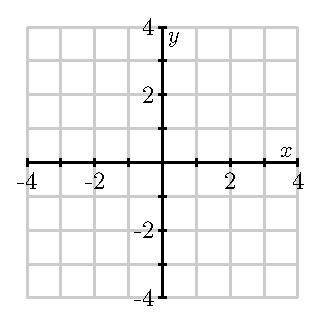
\includegraphics{empty-4.eps}
    
  \item Explain how we know that there is a nonzero solution to the
    homogeneous equation $A\xvec=\zerovec$.
    
    \vs{1}
    
  \item Find a nonzero solution to the homogeneous solution
    $A\xvec=\zerovec$.
    
    \vs{1}
  \item Use this solution to express one of the vectors as a linear
    combination of the others.
    
    \vs{1}
  \end{enumerate}
  
\item
  \begin{enumerate}[label=(\alph*)]
  \item What condition on a matrix $A$ will guarantee that its columns
    are linearly independent?

    \vs{1}
  \item Suppose that $\vvec_1,\vvec_2,\ldots,\vvec_n$ are linearly
    independent vectors in $\real^9$.  What can you say about the
    number of vectors in this set?

    \vs{1}
  \item What is the smallest number of vectors that can span
    $\real^{13}$?

    \vs{1}
  \item What is the largest number of vectors in $\real^{13}$ that are
    linearly independent?

    \vs{1}
  \item Suppose that a set of vectors in $\real^{13}$ is linearly
    independent and spans $\real^{13}$.  What can you say about the
    number of vectors?

    \vs{1}
  \end{enumerate}
  

    

  

\end{enumerate}


\end{document}
